\subsection{Desarrollo de la etapa de huevo}
Para el análisis de la tasa de desarrollo, en días, del huevo de Aedes aegypti, se incluyeron
los huevos que se desarrollaron completamente para pasar a ser una larva. Con el fin de realizar
una comparativa con los resultados obtenidos, en la tabla \cite{tab:desarrollo-huevo-test} se
utiliza como referencia los resultados obtenidos por \cite{BESERRA2006}, donde se presentan los
requerimientos térmicos para el desarrollo del aedes aegypti en condiciones naturales, para 5
cepas de Aedes Aegyti, provenientes de diferentes  poblaciones, a 5 temperaturas constantes
(18-34\textcelsius).

En la Figura \ref{fig:desarrollo-huevo-baserra2006}, se puede observar una compartiva con los
valores observados en \cite{BESERRA2006}, la media predicha y la media obtenida. En general se
obtuvo un desarrollo de $3.29$ días a 4 temperaturas constantes (22, 26, 30, 34 \textcelsius), con
una diferencia de, $0,97$, $0,87$, $0,87$, $1,15$ y $0,57$ días con la media general de los
valores observados en \cite{BESERRA2006} para las poblaciones de Boqueirão, B. dos Santos, C.
Grande, Itaporanga y Remígio respectivamente. Los autores de \cite{BESERRA2006}, señalan que a
18 \textcelsius, no existe desarrollo embrionario para las poblaciones de B. dos Santos, C. Grande
y Remígio, por lo que estos resultados no fueron incluidos en el calculo de la media general. En
relación a la media predicha, que fue obtenida mediante el modelo de \cite{sharpe1977reaction}, se
obtuvo una diferencia de $0,32$ días con la media obtenida.

\begin{table}
    \begin{minipage}{\textwidth}

        \caption{\label{tab:desarrollo-huevo-test} Análisis de la tasa de desarrollo, en días, de
        los huevos de Aedes aegypti a cinco temperaturas constantes (18-34 \textcelsius).}

        \begin{tabular}{p{5cm} c c c c c c }
            \hline \\
            Población    &18 \textcelsius & 22 \textcelsius & 26 \textcelsius & 30 \textcelsius & 34 \textcelsius & Media General\\

            \hline
            \hline \\
            Boqueirão            & 9,3 $^{b}$  & 6,5  & 3,9  & 3,3  & 3,5  & 4,3  \\
            B. dos Santos        & -- $^{a}$   & 5,9  & 4,3  & 3,7  & 2,9  & 4,2  \\
            C. Grande            & -- $^{a}$   & 5,5  & 3,4  & 4,4  & 3    & 4,07 \\
            Itaporanga           & 9,2 $^{b}$  & 6,2  & 4,7  & 3,1  & 3,5  & 4,38 \\
            Remígio              & -- $^{a}$   & 6    & 4,5  & 2    & 2,5  & 3.75 \\
            Media Predicha$^{c}$ & 6.61 $^{b}$ & 5,1  & 3.9  & 3.03 & 2.37 & 3.6  \\
            Media Obtenida$^{d}$ & 6.08 $^{b}$ & 5.06 & 3.03 & 3.03 & 2.02 & 3.29 \\

        \end{tabular}
        \footnotetext[1]{No hubo desarrollo embrionario a 18\textcelsius, \cite{BESERRA2006}.}
        \footnotetext[2]{Como no hubo desarrollo embrionario en las demas poblaciones a 18\textcelsius,
        se decidió no incluir estos datos en la media general, sólo representa el promedio para
        estas poblaciones \cite{BESERRA2006}.}
        \footnotetext[3]{Resultados obtenidos por el modelo de Sharpe \& DeMichele.}
        \footnotetext[4]{Resultados obtenidos mediante el proceso evolutivo.}
    \end{minipage}
\end{table}


\begin{figure}
\begin{minipage}{\textwidth}
    \begin{tabular}{c c }
        \initbox
        \num\putindeepbox[7pt]{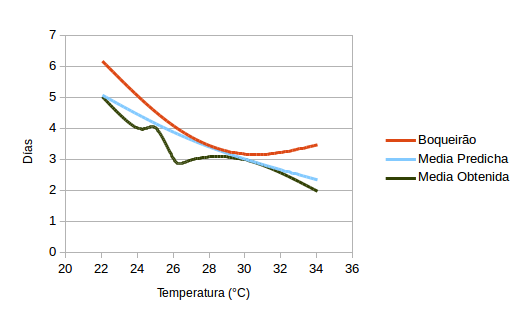
\includegraphics[width=0.4\textwidth]{capitulo-6/graphics/desarrollo-huevos-1.png}} &
        \num\putindeepbox[7pt]{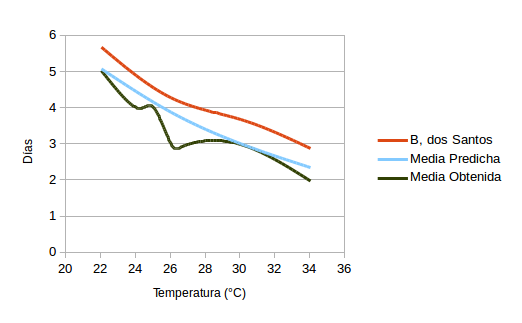
\includegraphics[width=0.4\textwidth]{capitulo-6/graphics/desarrollo-huevos-2.png}} \\

        \num\putindeepbox[7pt]{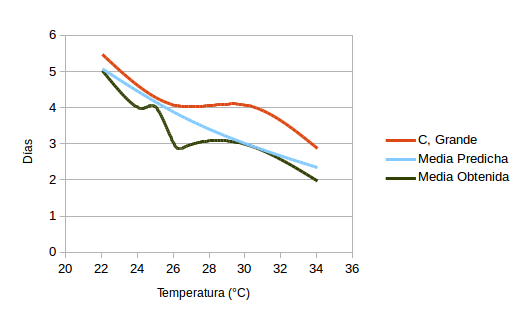
\includegraphics[width=0.4\textwidth]{capitulo-6/graphics/desarrollo-huevos-3.png}} &
        \num\putindeepbox[7pt]{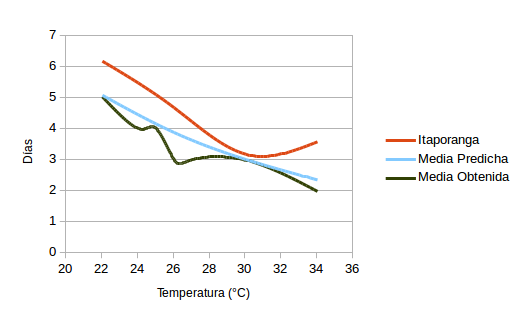
\includegraphics[width=0.4\textwidth]{capitulo-6/graphics/desarrollo-huevos-4.png}} \\

        \num\putindeepbox[7pt]{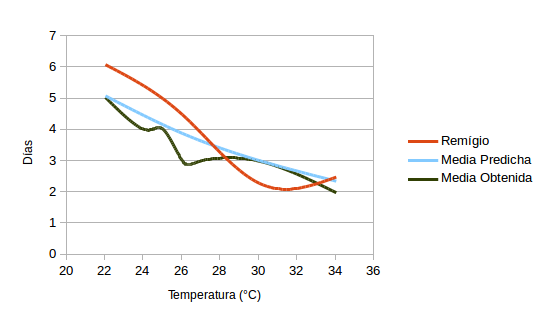
\includegraphics[width=0.4\textwidth]{capitulo-6/graphics/desarrollo-huevos-5.png}} &
        \num\putindeepbox[7pt]{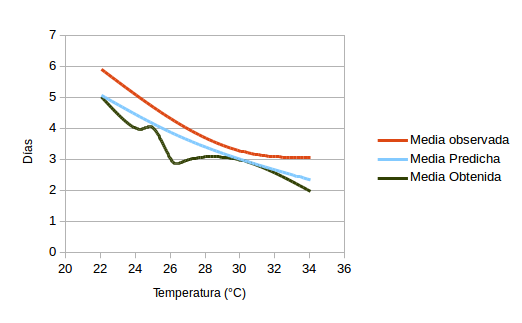
\includegraphics[width=0.4\textwidth]{capitulo-6/graphics/desarrollo-huevos-6.png}} \\
    \end{tabular}

    \caption{\label{fig:desarrollo-huevo-baserra2006}
    Comparativa entre ,la media obtenida, la media predicha y las medias observadas por \cite{
    BESERRA2006} en distintas pobalciones a 4 temperaturas contantes (18-34 \textcelsius) para
    las tasas de desarrollo de los huevos del Aedes Aegypti.}

    \footnotetext[1]{Tasa de desarrollo de Boqueirão en comparación con la media predicha y obtenida.}
    \footnotetext[2]{Tasa de desarrollo de B. dos Santos en comparación con la media predicha y obtenida.}
    \footnotetext[3]{Tasa de desarrollo de C. Grande en comparación con la media predicha y obtenida.}
    \footnotetext[4]{Tasa de desarrollo de Itaporanga en comparación con la media predicha y obtenida.}
    \footnotetext[5]{Tasa de desarrollo de Remígio en comparación con la media predicha y obtenida.}
    \footnotetext[6]{Media observada en los poblados de Boqueirão, B. dos Santos, C. Grande, Itaporanga, Remígio en comparación con la media predicha y obtenida.}

\end{minipage}
\end{figure}
